\subsection{University of Uzbekistan}

Para esta medición se eligió la Universidad Nacional de Uzbekistan (O'zbekiston Milliy Universiteti), ubicada en Tashkent, Uzbekistan. El \emph{host} correspondiente a esta universidad es \emph{nuu.uz}.\par
Para esta medición se espera que la ruta se divida en tres tramos siendo el primer tramo el correspondiente a Argentina-EEUU, cruzando el Océano Atlántico hasta desembocar en Europa y finalmente desde Europa hacia el Oeste de Asia alcanzando finalmente Uzbekistan.\par
Las mediciones fueron realizadas en repetidas ocasiones con el objetivo de no caer en conclusiones precipitadas, utilizando en cada oportunidad 30 iteraciones por TTL. Finalmente los RTTs conseguidos fueron los siguientes: \\
\begin{figure}[H]
    \centering
    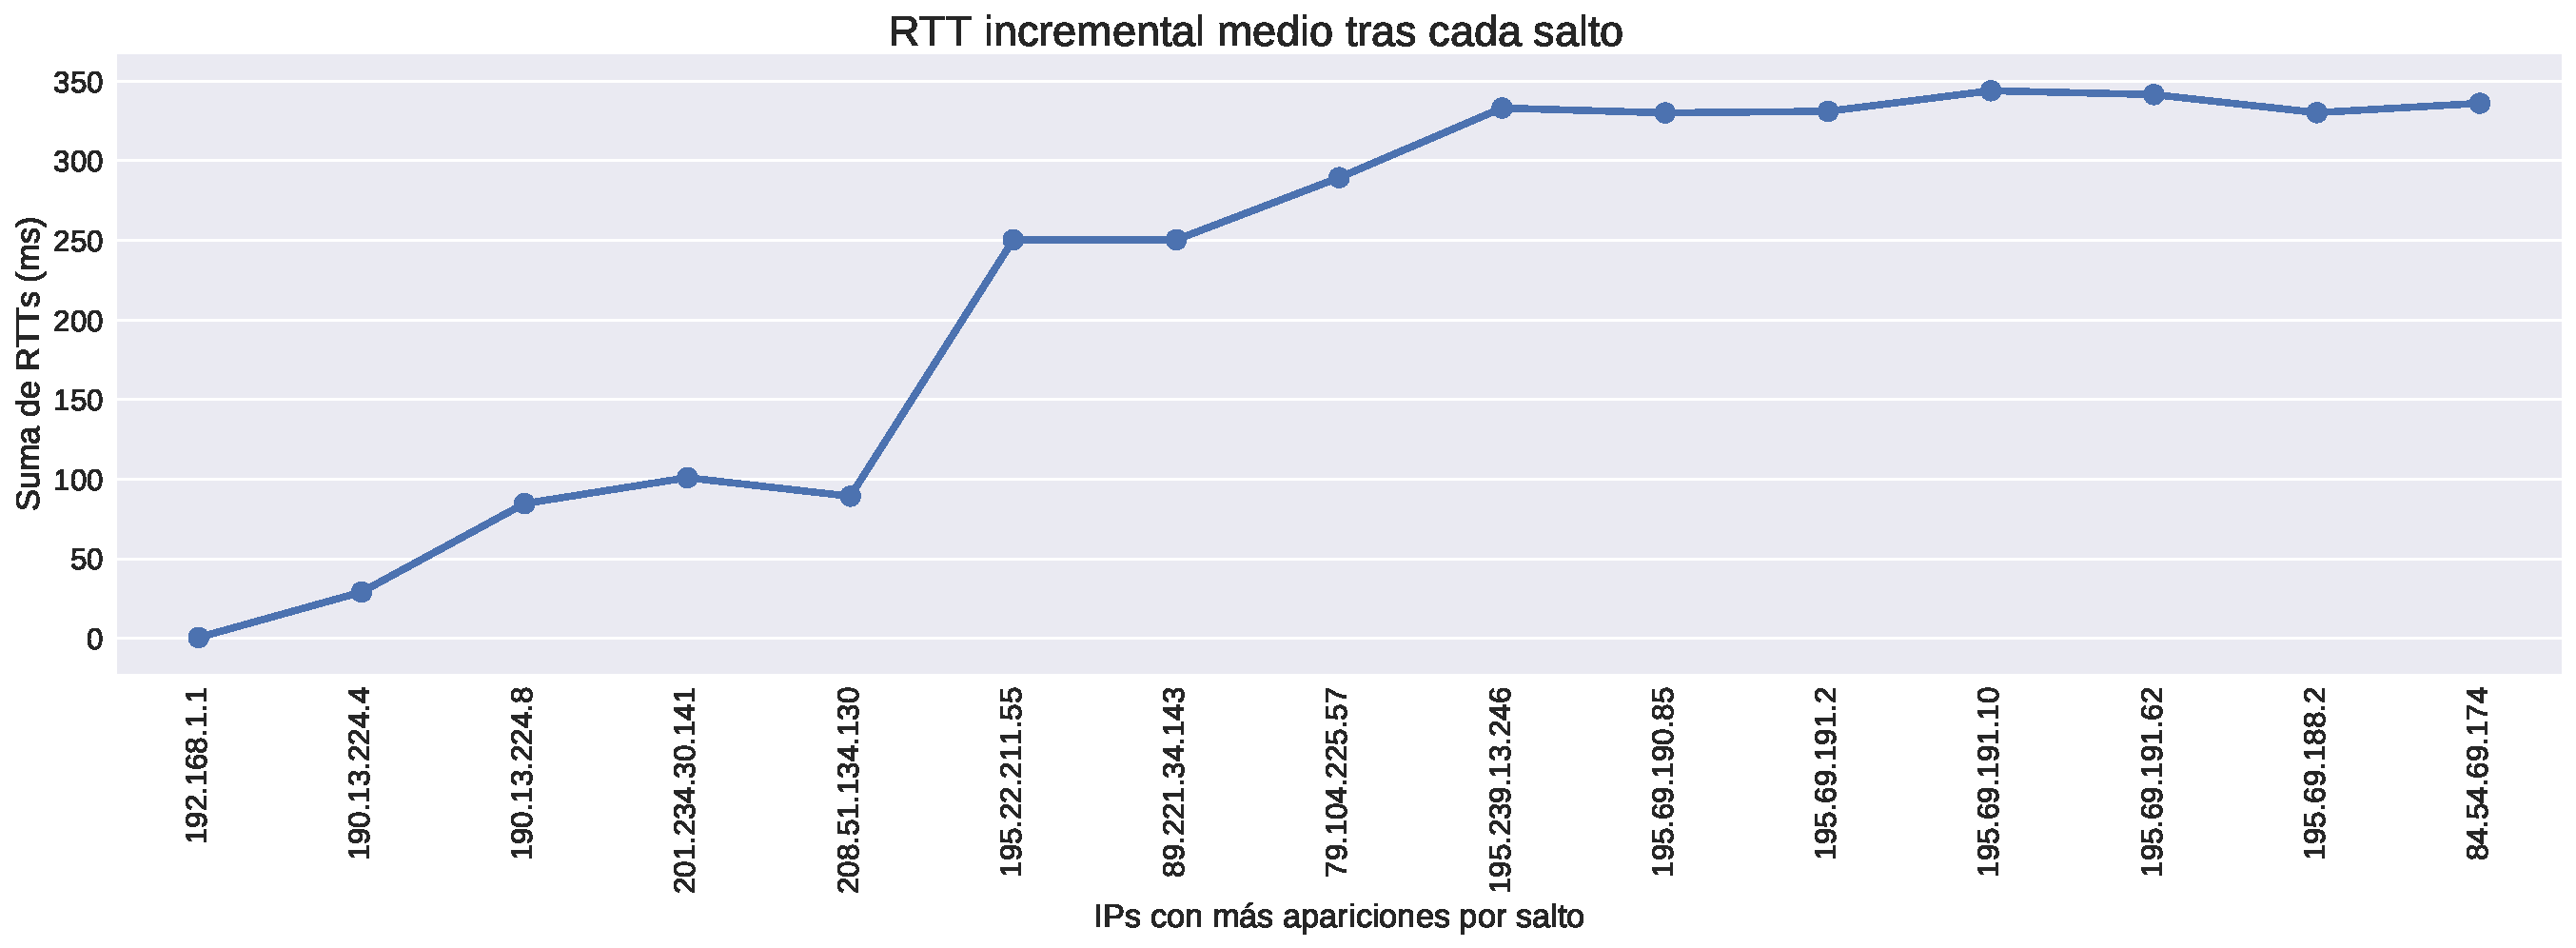
\includegraphics[width=1\textwidth, height=1\textheight, keepaspectratio]{../img/nuu-uz-incrementales}
    \caption{Comportamiento incremental de RTTs medios medidos.}
    \label{fig:nuu-uz-incrementales}
\end{figure}
En el gráfico se pueden observar dos incrementos notorios en el RTT, el primer incremento se corresponde con el tramo transatlántico que une EEUU con Europa, debido a que este es el tramo más largo.\par
A continuación se nota otro incremento aunque no tan notorio en el RTT seguido de un incremento más paulatino, casi constante. Este pequeño incremento nos predispone a considerar la existencia de un cuarto tramo y reconsiderar la idea inicial en la que el ultimo tramo es desde un único país Europeo hasta Uzbekistan.\par


\begin{figure}[H]
   \centering
       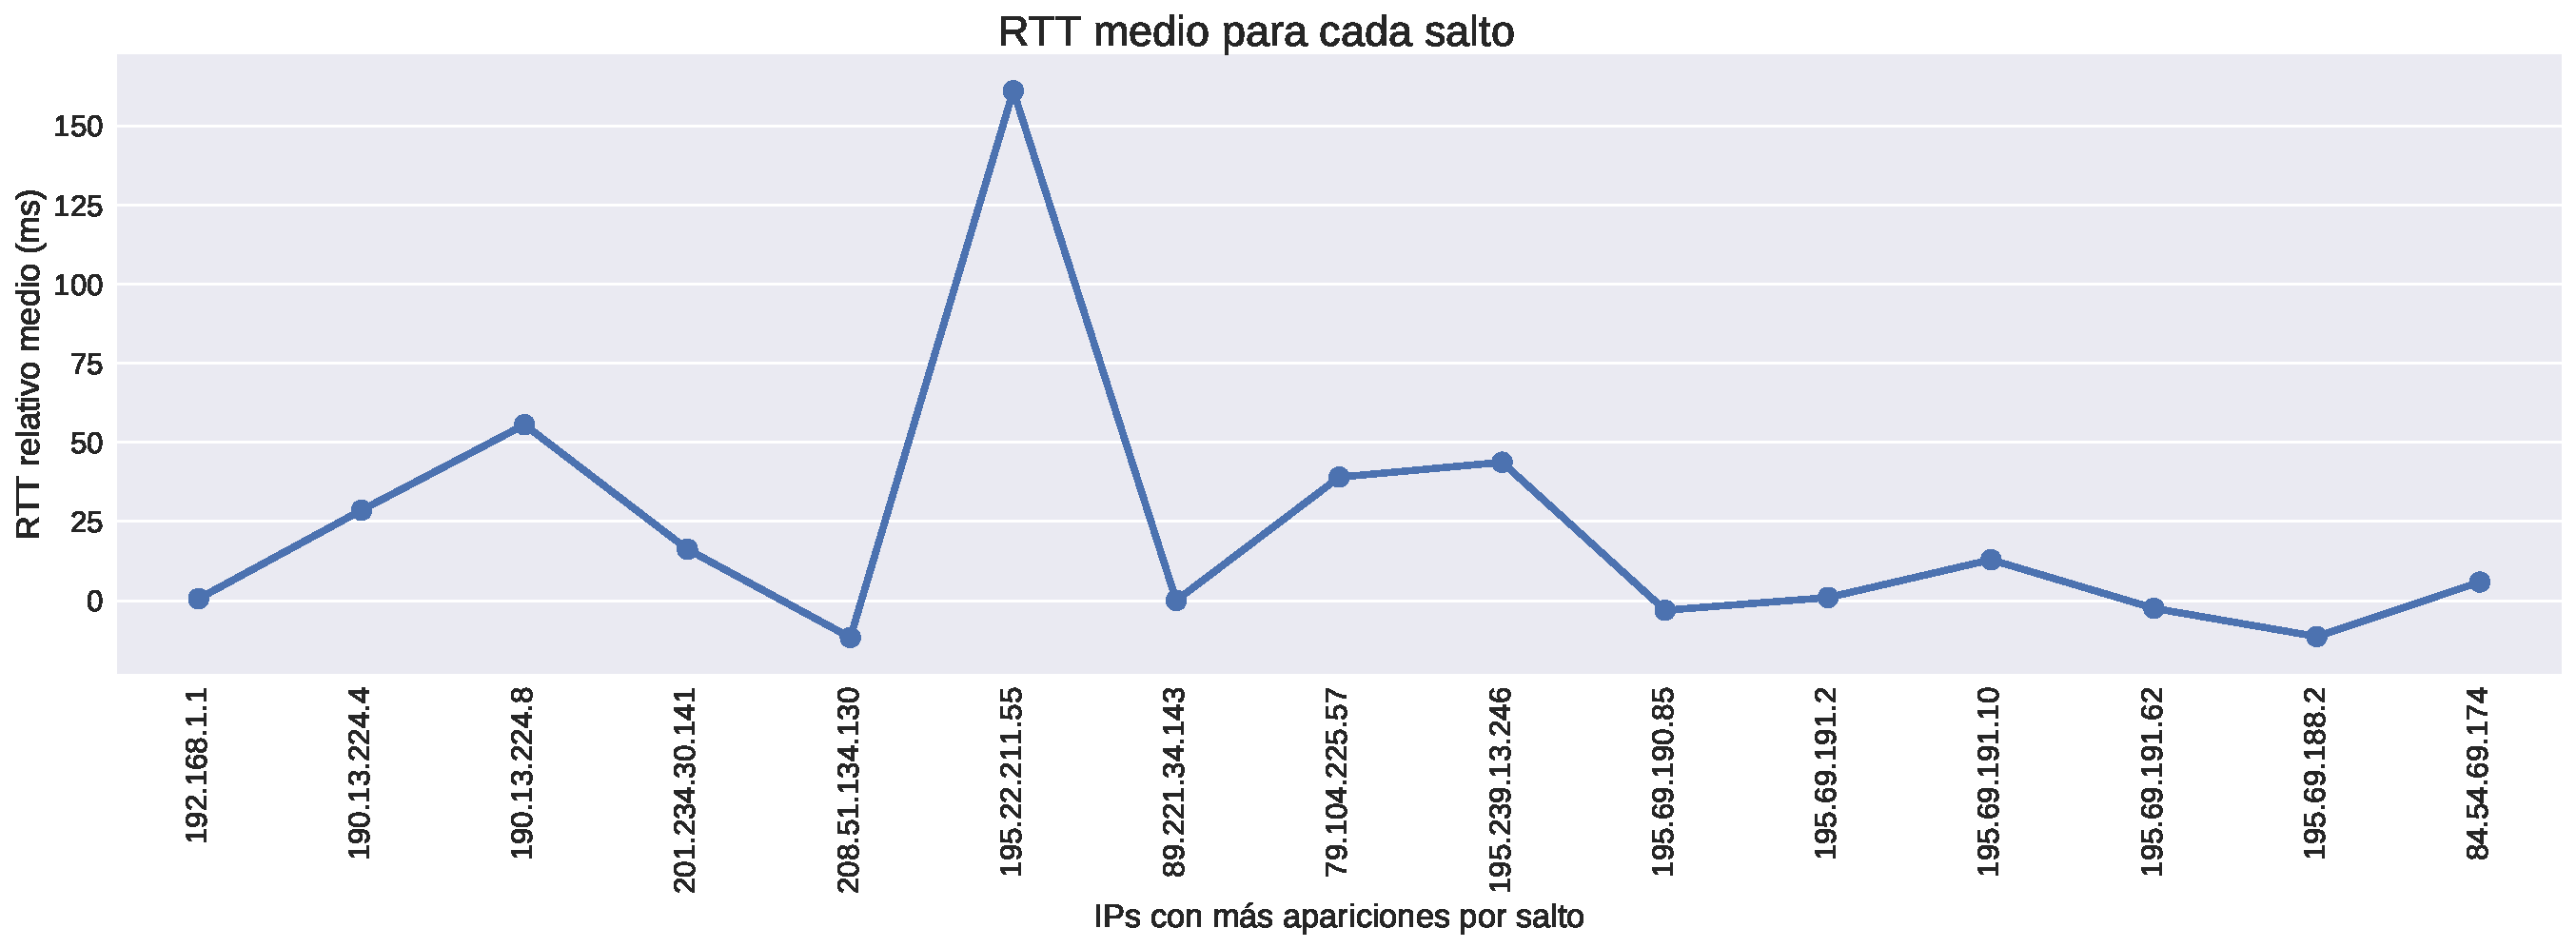
\includegraphics[width=1\textwidth, height=1\textheight, keepaspectratio]{../img/nuu-uz-rtts}
 \caption{RTTs medios medidos para una traceroute a la Universidad de Uzbekistan.}
 \label{fig:nuu-uz-rtts}
\end{figure}

Buscando información de la IP '195.22.211.55' pudimos observar que se trata de un host ubicado en Roma, Italia. Debido al incremento en el RTT medio medido para esta IP, creemos que éste es país europeo en el cual desemboca el tramo transatlántico antes de seguir rumbo hacia su destino. \par

Por otro lado, el incremento presente en '195.239.13.246', se corresponde con un host ubicado en Moscú, Rusia y es el que funciona como enlace entre Europa y Asia dándonos de este modo el cuarto tramo del recorrido.\par

\begin{figure}[H]
   \centering
       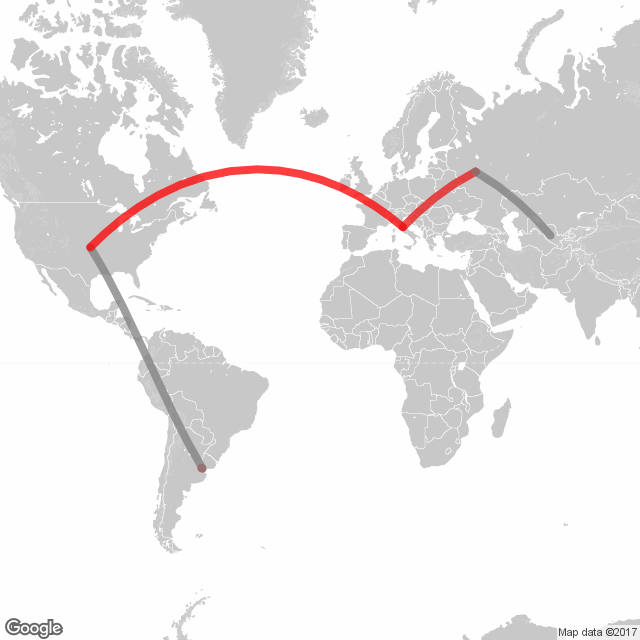
\includegraphics[width=0.5\textwidth, keepaspectratio]{../img/nuu-uz-map}
 \caption{Mapa de ubicaciones inferidas para una traceroute a la Universidad de Uzbekistan.}
 \label{fig:nuu-uz-map}
\end{figure}


Finalmente, graficando la ruta obtenida podemos constatar que efectivamente el recorrido consta de cuatro tramos, siendo los tramos EEUU-Italia el tramo con más RTT seguido del tramo Italia-Rusia y los responsables de los picos observados en los gráficos anteriores. Considerando este gráfico podemos concluir que exite un total de 3 saltos intercontinentales (América-Europa-Asia) a pesar del tramo que une a Italia con Moscú que si bien se trata de un tramo con un RTT considerable no es un tramo intercontinental.\par

En esta medición asi como en las anteriores, se puede ver la misma anomalía en la que se utiliza la totalidad de los 30 \emph{Hoops} sin poder determinar con seguridad en qué salto se llega al host destino. Teniendo esto en cuenta y que la cantidad de nodos que responden al \emph{time-exceeded} es 15, se puede concluir que solo el 50\% de los nodos respondió al \emph{echo-request} si contamos esta vez contra los 30 saltos máximo totales (la otra opción sería contar el último salto que responde \emph{time-exceeded} como el destino, aunque no se pueda determinar si realmente lo es, como hicimos antes).


\begin{figure}[H]
   \centering
       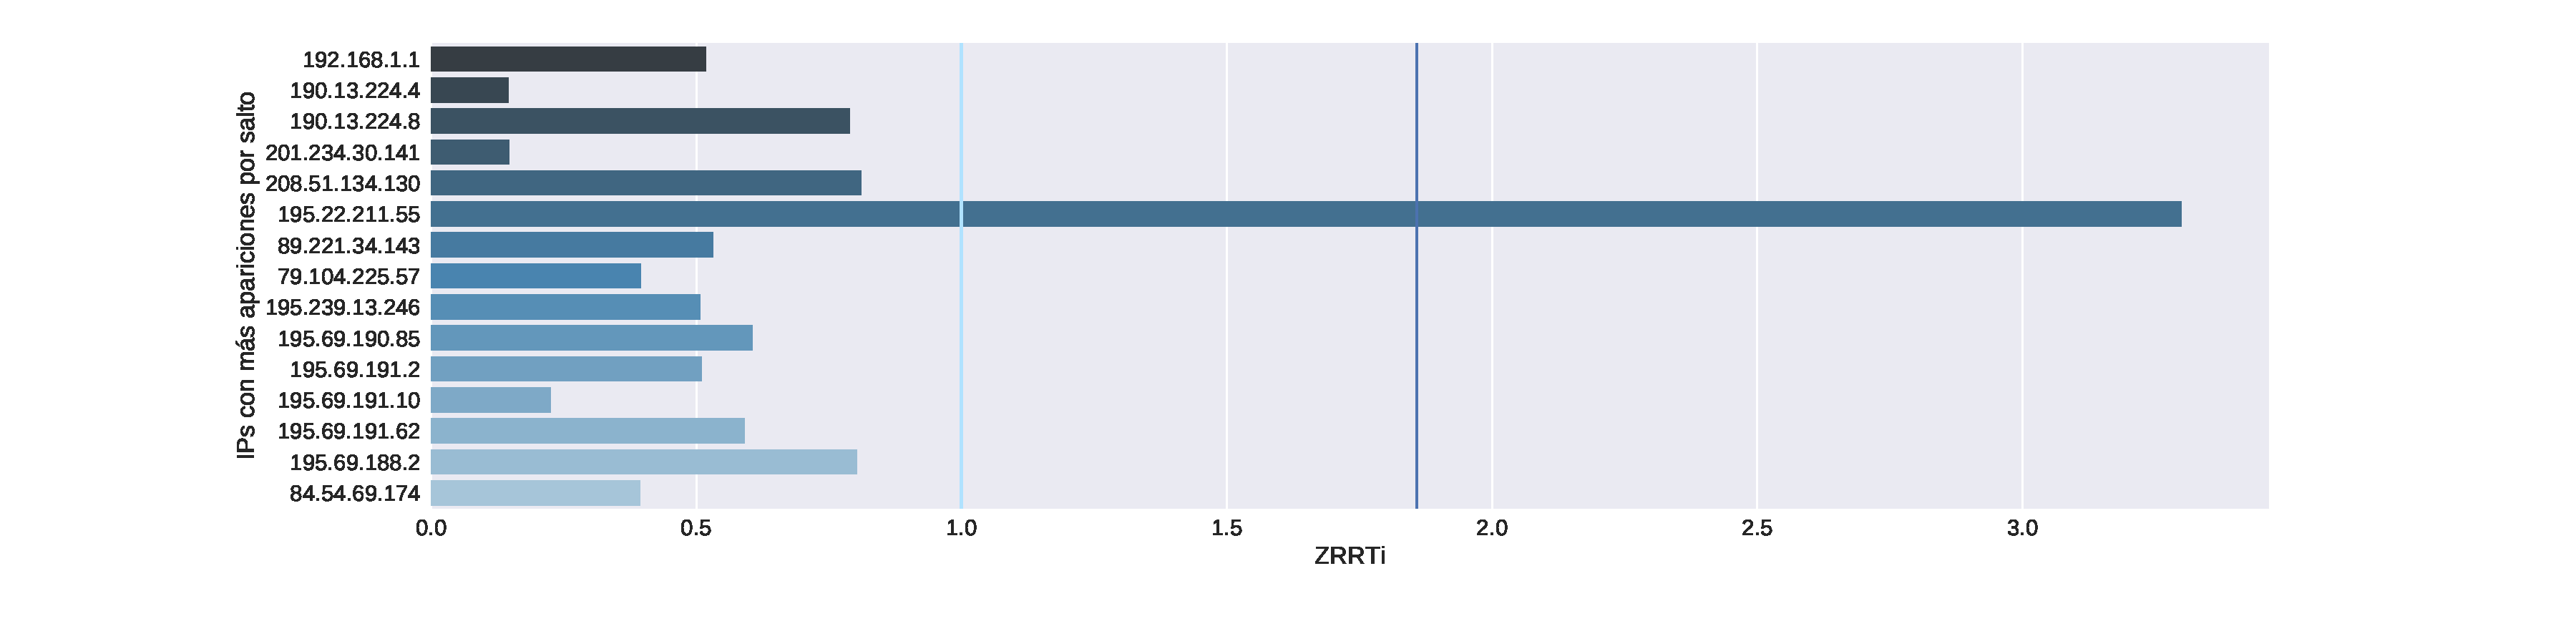
\includegraphics[width=1\textwidth, height=1\textheight, keepaspectratio]{../img/nuu-uz-zrtt}
 \caption{Outliers de la distribución ZRRTi según el método de Cimbala. En azul oscuro: valor $ZRTT_i$ correspondiente a $\tau(n)$ con $n$ el largo de ruta y un alfa fijo (0.05 sugerido en el paper de referencia).}
 \label{fig:nuu-uz-zrtt}
\end{figure}

En la figura \ref{fig:nuu-uz-zrtt} se ven los outliers de la muestra. Respecto del umbral de la tabla $\tau$. Se distingue un solo outlier correspondiente al nodo ubicado en Italia. Esto resultado es esperado debido a que se trata del extremo Europeo del tramo transatlántico alcanzando de este modo el RTT máximo de la medición sobrepasando incluso a los demás tramos intercontinentales y etiquetando a éstos últimos como falsos negativos.
